\documentclass[11pt,a4paper]{article}

\usepackage[utf8]{inputenc}
\usepackage[T1]{fontenc}
\usepackage[margin=2.5cm]{geometry}
\setlength{\headheight}{14pt}
\usepackage[colorlinks=true,linkcolor=red!60!black,urlcolor=blue!60!black,citecolor=blue!60!black]{hyperref}
\usepackage{xcolor}
\usepackage{booktabs}
\usepackage{listings}
\usepackage{enumitem}
\usepackage{titlesec}
\usepackage{parskip}
\usepackage{microtype}
\usepackage{fancyhdr}
\usepackage{tabularx}
\usepackage{tikz}
\usetikzlibrary{positioning, arrows.meta, fit, backgrounds}

\definecolor{usydred}{HTML}{C63B1E}
\definecolor{ochre}{HTML}{C4972A}
\definecolor{sandstone}{HTML}{E8D5B5}
\definecolor{charcoal}{HTML}{2D2926}
\definecolor{eucalypt}{HTML}{567D46}
\definecolor{codebg}{HTML}{F5F0E8}
\definecolor{mutedtext}{HTML}{6B6560}

\titleformat{\section}{\Large\bfseries\color{usydred}}{\thesection}{1em}{}
\titleformat{\subsection}{\large\bfseries\color{charcoal}}{\thesubsection}{1em}{}

\lstdefinestyle{code}{
  basicstyle=\ttfamily\small,
  backgroundcolor=\color{codebg},
  frame=single,
  framesep=6pt,
  rulecolor=\color{sandstone},
  breaklines=true,
  keywordstyle=\color{usydred},
  commentstyle=\color{mutedtext}\itshape,
  stringstyle=\color{ochre},
  numbers=none,
  showstringspaces=false,
  upquote=true,
}
\lstset{style=code}

\pagestyle{fancy}
\fancyhf{}
\fancyhead[L]{\textcolor{mutedtext}{\small DASH Repository: Phase 1 Deployment at USyd}}
\fancyhead[R]{\textcolor{mutedtext}{\small \thepage}}
\renewcommand{\headrulewidth}{0pt}

\title{\vspace{-2cm}\textcolor{usydred}{\rule{\textwidth}{4pt}}\\[1em]
\Huge\bfseries Deploying the DASH Repository at USyd\\[0.4em]
\large\mdseries\color{mutedtext} Phase 1 technical analysis}
\author{\small Charles Perkins Centre, Data Science Hub \\ \small University of Sydney}
\date{10 May 2026}

\begin{document}
\maketitle
\thispagestyle{empty}
\vspace{1em}

\begin{quote}
\itshape\color{mutedtext}\small
This document analyses what it would take to move the DASH Repository from a working prototype into a system that USyd researchers can actually use. It is written for project supervisors and assumes technical literacy but no prior familiarity with MongoDB, vector embeddings, or specific USyd infrastructure.
\end{quote}

\vspace{1em}

\section{Where we are now}

The DASH Repository, in its current prototype form, is a working search system for past DASH consultation reports. A researcher types a query in plain English (for example, \emph{skin proteomics}) and receives a ranked list of relevant past projects. The matching is done by meaning rather than keywords: a query for \emph{skin proteomics} also retrieves a project filed under \emph{dermatology, mass spectrometry}, because those phrases describe the same kind of work in different vocabulary. The prototype lives across four pieces, illustrated below. Today, all four run from a developer's laptop and two external cloud accounts.

\medskip

\begin{center}
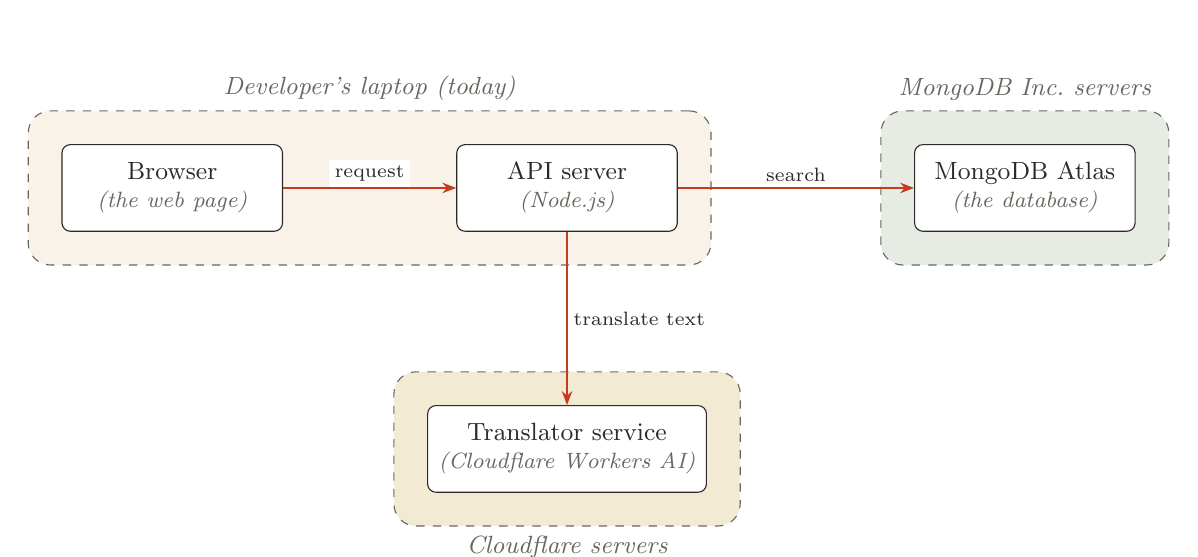
\begin{tikzpicture}[
  every node/.style={font=\small, text=charcoal},
  component/.style={
    draw=charcoal,
    rounded corners=3pt,
    minimum width=2.8cm,
    minimum height=1.1cm,
    fill=white,
    align=center,
    inner sep=4pt,
  },
  loclabel/.style={
    font=\small\itshape,
    text=mutedtext,
  },
  link/.style={
    -{Stealth[length=5pt]},
    thick,
    draw=usydred,
  },
  arrowlabel/.style={
    font=\scriptsize,
    text=charcoal,
    inner sep=2pt,
    fill=white,
  },
]
  \node[component] (browser) {Browser \\[-1pt] {\footnotesize\itshape\color{mutedtext}(the web page)}};
  \node[component, right=2.2cm of browser] (server) {API server \\[-1pt] {\footnotesize\itshape\color{mutedtext}(Node.js)}};
  \node[component, right=3.0cm of server] (atlas) {MongoDB Atlas \\[-1pt] {\footnotesize\itshape\color{mutedtext}(the database)}};
  \node[component, below=2.2cm of server] (cf) {Translator service \\[-1pt] {\footnotesize\itshape\color{mutedtext}(Cloudflare Workers AI)}};

  \begin{scope}[on background layer]
    \node[draw=mutedtext, dashed, rounded corners=8pt, inner sep=12pt,
          fill=sandstone!30,
          fit=(browser) (server),
          label={[loclabel]above:Developer's laptop (today)}] {};
    \node[draw=mutedtext, dashed, rounded corners=8pt, inner sep=12pt,
          fill=eucalypt!15,
          fit=(atlas),
          label={[loclabel]above:MongoDB Inc.\ servers}] {};
    \node[draw=mutedtext, dashed, rounded corners=8pt, inner sep=12pt,
          fill=ochre!20,
          fit=(cf),
          label={[loclabel]below:Cloudflare servers}] {};
  \end{scope}

  \draw[link] (browser) -- node[arrowlabel, above]{request} (server);
  \draw[link] (server) -- node[arrowlabel, above]{search} (atlas);
  \draw[link] (server) -- node[arrowlabel, right]{translate text} (cf);
\end{tikzpicture}
\end{center}

\smallskip
\noindent{\small\itshape\color{mutedtext} The four pieces of the DASH Repository, grouped by where they run today. The companion \emph{MongoDB Implementation Primer} explains each in detail; this document is concerned with where each piece would live in a USyd-deployed version.}

\medskip

The question this document answers is straightforward: what changes when the system stops being a demo on a developer's laptop and starts being something USyd researchers actually use? The remaining sections set out the scope of Phase 1, the four questions worth answering before deployment, three concrete deployment options, a recommendation, and the open items requiring supervisor or ICT input.

\section{Scope of Phase 1}

The single most important decision in Phase 1 is the access model, because it determines everything downstream. The proposed model is:

\begin{quote}
\textbf{Public by default, with opt-out.} Every project added to the repository is, by default, viewable by anyone on the internet. During intake, the collaborator is offered the explicit option to mark their project as not public; in that case the project is held back from the search results and never appears in responses. The expectation in Phase 1 is that the substantial majority of projects will be public.
\end{quote}

This single decision has three immediate consequences for the deployment.

\paragraph{No authentication is required for Phase 1.} Because the search service is open to the public, there is no need to integrate with Unikey or Microsoft Entra ID, no need to manage user accounts, and no need to run a session layer. The role-based access control (RBAC) machinery already built into the prototype remains in place but sits idle until the first opt-out project arrives, at which point it activates without further engineering work. This deferral is the single largest source of simplification in the Phase 1 deployment.

\paragraph{Cost and abuse become a real concern.} A public API can be called by anyone, including bots and other automated traffic. The translator service (Cloudflare Workers AI) charges per call, so an unrestricted public endpoint is also an unrestricted billing surface. The deployment must include a basic per-IP rate limit (for example, 30 queries per minute per IP) to bound the worst case. This is straightforward to implement and is assumed in every deployment option below.

\paragraph{The four questions that remain.} With identity removed from the critical path, the questions that still need answering before deployment are: \emph{where does each piece run}, \emph{where does the data physically live}, \emph{what does it cost}, and \emph{who owns it operationally?} Section 3 takes each in turn.

\section{The four questions}

With identity off the critical path, four questions remain. Each is addressed below in its own short subsection ending with a clear recommendation. The concrete deployment options that combine the answers across all four are the subject of section 4.

\subsection{Where each piece runs}

The system has four pieces (figure 1). The web page is small and can be bundled with the API server or served from a free static-site host. The API server is a single Node.js process and runs comfortably on a small virtual machine. The database is already on a managed service (MongoDB Atlas) and there is no operational reason to move it in Phase 1. The translator service runs on Cloudflare Workers AI and would need a non-trivial GPU to self-host effectively. The interesting choice is therefore where the API server lives. Three options are realistic: a USyd-hosted virtual machine (managed by ICT or provisioned within CPC's own infrastructure), the Nectar Research Cloud (subject to USyd researcher access), or a small commercial cloud VM in the Sydney AWS or Azure region. The first option is operationally the simplest if it can be arranged, because patches, backups, and uptime monitoring fall under existing institutional processes rather than the lead developer's personal workflow.

\paragraph{Recommendation.} Host the API server on a USyd-hosted virtual machine if one can be obtained from ICT or CPC. Failing that, fall back to the Nectar Research Cloud (free, subject to USyd researcher access), or to a small commercial cloud VM in the Sydney AWS or Azure region. Bundle the static web page with the API server in all cases. Leave the database on MongoDB Atlas and the translator on Cloudflare Workers AI; self-hosting either of these is a Phase 2 question.

\subsection{Where the data lives}

Even though all project documents are public under the Phase 1 access model, the \emph{search logs} collection is not: it records what researchers are looking for, which is meaningful context about how DASH and CPC are being used. Project documents, embeddings, and search logs all live in MongoDB Atlas, in whichever cloud region the cluster was deployed. The translator service runs at Cloudflare's network edge (which has Australian points of presence); Cloudflare's policy is that inputs to inference endpoints are not retained beyond the request itself.

\paragraph{Recommendation.} Confirm that the Atlas cluster is deployed in the Sydney AWS region (\texttt{ap-southeast-2}). If it is not, migrate it. This places all DASH project data and search logs on Australian infrastructure at no additional cost, and pre-empts the question if it is ever raised by the USyd research-data office.

\subsection{Cost}

The Phase 1 monthly cost is small and dominated by two choices: which Atlas tier carries the database, and where the API server is hosted. The remaining three line items (the embedding service, basic rate limiting, and the domain name) are too small at Phase 1 scale to move the total in a meaningful way. This subsection models the cost across the full Phase 1 trajectory.

\paragraph{Two scenarios.} The costs below are modelled for two operating points along the Phase 1 trajectory. \emph{Phase 1 launch} assumes around 100 projects in the catalogue and roughly 150 agent queries per month, representing the first credible deployment with all DASH analysts contributing. \emph{Phase 1 mature} assumes around 1{,}000 projects and roughly 900 queries per month, representing late Phase 1 when the catalogue holds substantial back-content and CPC awareness has spread. Both points fit comfortably inside Phase 1 cost behaviour: as the next sections show, no line item changes category between the two.

\paragraph{Where the API server runs.} Four realistic options exist for hosting the API server, ordered from highest to lowest institutional ownership. All four are appropriate for the small, long-running Node.js process the API server is in Phase 1; the differences are operational rather than performance-related.

\begin{enumerate}[leftmargin=1.5em,itemsep=4pt]
  \item \textbf{ICT-managed virtual machine.} The University of Sydney ICT service catalogue (knowledge-base article KB0010875) lists a small dedicated VM environment intended for hosting websites, applications, and databases. ICT's public policy is that ongoing hardware management is provided at no charge; setup and any hardware purchased on the researcher's behalf may be chargeable. Treat this option as \emph{\$0 per month base, plus an unknown one-off setup fee}, contingent on ICT confirming both eligibility and a suitable VM size for a small public-facing Node.js process. This is the institutionally cleanest path if it can be arranged.
  \item \textbf{Sydney Informatics Hub subsidised support.} SIH offers fully subsidised research support and computing for researchers holding active competitive grant funding. The DASH JMRF grant qualifies. Applications were called in early 2026 with outcomes announced mid-March 2026; the scheme is expected to recur annually. If a SIH allocation can be obtained, the API server runs at no marginal cost, with patches and monitoring under SIH's operational umbrella. The annual application window is the key constraint: missing it pushes the option to the following cycle.
  \item \textbf{ARDC Nectar Research Cloud.} The Australian national research cloud is free to Australian researchers via Australian Access Federation (AAF) login. Six-month trial allocations convert to 12-month allocations with renewals. An \texttt{m3.small} flavour (2 vCPU, 4 GB RAM, 30 GB root disk) covers the API server with substantial headroom. Suitable as a fallback if no USyd-internal VM is available.
  \item \textbf{RONIN Cloud (USyd-managed AWS) or commercial cloud.} RONIN provides USyd researchers with a managed abstraction over AWS, with consumption flowing through institutional billing. A \texttt{t3.small}-class VM in the Sydney AWS region (\texttt{ap-southeast-2}) costs roughly AUD \$15 per month. A direct commercial cloud VM in the same region sits in the same range. This is the most operationally familiar but the only consistently paid option.
\end{enumerate}

\paragraph{Database tier.} The earlier prototype work assumed the Atlas M0 free tier was suitable for Phase 1, on the basis of its 512 MB storage allowance. That allowance comfortably holds the projected document volume (around 16 MB of project documents and embeddings at 1{,}000 projects, plus around 50 MB per year of query logs). However, MongoDB has clarified in 2025 that Atlas Vector Search is not recommended on M0: index operations must be performed manually through the Atlas UI, and the shared resources are not suited to production query traffic. The appropriate Phase 1 tier is therefore the newer \emph{Atlas Flex} (generally available February 2025), which supports Atlas Vector Search natively, includes 5 GB of storage, and is priced on a pay-as-you-go basis between AUD \$8 and \$30 per month with a hard \$30 monthly cap.

\paragraph{Embedding service.} Cloudflare Workers AI prices the \texttt{bge-small-en-v1.5} embedding model at USD \$0.020 per million input tokens, with a free daily neuron allocation that absorbs small applications entirely. The Phase 1 mature scenario generates roughly 90{,}000 query tokens per month and an occasional bulk re-embedding pass of around 800{,}000 tokens for the full catalogue: total monthly cost is well under one Australian cent. This component is effectively free at Phase 1 scale and is included in the tables below only for completeness.

\paragraph{Smaller line items.} A custom domain name (for example \texttt{dash.cpc.usyd.edu.au} via ICT, or a \texttt{.org.au} purchased directly) costs around AUD \$15 per year, or \$1.25 per month. Basic per-IP rate limiting is available within Cloudflare's free tier and adds nothing to the bill.

\medskip

\noindent\textbf{Phase 1 launch: around 100 projects, around 150 queries per month.}

\medskip

\noindent\begin{tabularx}{\textwidth}{X r}
\toprule
\textbf{Component} & \textbf{Monthly cost (AUD)} \\
\midrule
API server hosting (ICT VM, SIH, or Nectar) & \$0 \\
API server hosting (RONIN or commercial fallback) & \$15 \\
MongoDB Atlas (Flex tier, pay-as-you-go) & \$8 to \$15 \\
Cloudflare Workers AI embeddings & \textless\,\$0.01 \\
Cloudflare rate limiting (free tier) & \$0 \\
Domain name & \$1.25 \\
\midrule
\textbf{Total, best case (institutional hosting)} & \textbf{\$9 to \$16} \\
\textbf{Total, fallback (paid hosting)} & \textbf{\$24 to \$31} \\
\bottomrule
\end{tabularx}

\medskip

\noindent\textbf{Phase 1 mature: around 1{,}000 projects, around 900 queries per month.}

\medskip

\noindent\begin{tabularx}{\textwidth}{X r}
\toprule
\textbf{Component} & \textbf{Monthly cost (AUD)} \\
\midrule
API server hosting (ICT VM, SIH, or Nectar) & \$0 \\
API server hosting (RONIN or commercial fallback) & \$15 \\
MongoDB Atlas (Flex tier, near or at cap) & \$25 to \$30 \\
Cloudflare Workers AI embeddings & \textless\,\$0.05 \\
Cloudflare rate limiting (free tier) & \$0 \\
Domain name & \$1.25 \\
\midrule
\textbf{Total, best case (institutional hosting)} & \textbf{\$26 to \$31} \\
\textbf{Total, fallback (paid hosting)} & \textbf{\$41 to \$46} \\
\bottomrule
\end{tabularx}

\medskip

\paragraph{What the model implies.} Three observations follow. First, the Phase 1 trajectory from launch to mature moves the monthly bill by only about \$15: it is dominated by Atlas Flex moving from the floor of its band toward its cap. Second, the swing between institutional hosting and paid fallback is about \$15 per month and is similar at both endpoints, so the hosting decision can be made independently of how the catalogue grows. Third, no Phase 1 operating point sits above approximately AUD \$50 per month at the worst case, which keeps the system within an order of magnitude of zero throughout.

\paragraph{Phase 2 cost triggers.} Phase 1 cost behaviour ends at three explicit thresholds. The first is sustained query traffic that would exhaust Cloudflare's free embedding allowance, which begins to bite around 10{,}000 queries per month and would add roughly AUD \$0.20 per month per additional 10{,}000 queries: still small, but worth knowing. The second is Atlas Flex approaching its 5 GB storage allowance, which the storage model above suggests would occur somewhere around 50{,}000 projects or several years of accumulated query logs: not a Phase 1 concern. The third is the arrival of the first opt-out project, which activates RBAC, motivates authentication, and starts the Phase 2 conversation regardless of cost.

\paragraph{Recommendation.} Budget AUD \$30 per month for Phase 1 across the full launch-to-mature trajectory, with paid-hosting fallback raising the cap to \$50. Lead with an ICT-managed VM if institutional channels can be arranged within the deployment window; otherwise apply for the annual SIH allocation, with Nectar as the immediate fallback if neither lands in time. Start the database on the Atlas Flex tier rather than M0, accepting the \$8 to \$30 monthly band as the price of production-ready vector search.

\subsection{Operational ownership}

A deployed system is not a finished system. It needs someone to apply security patches, watch for outages, restore backups when needed, renew the domain, keep an eye on the Asana sync, and respond when researchers report that something is broken. Atlas's free tier does not include automated backups; the M10 paid tier does. A USyd-managed VM may bring the API server under ICT's patch and monitoring umbrella; a commercial cloud VM does not, and the responsibility falls to whoever set it up. The Asana sync is the quiet failure mode worth naming explicitly: it is a small piece of code that fails silently if the Asana API changes shape, and the only way to notice the failure is to look.

\paragraph{Recommendation.} Phase 1 operational ownership rests with the lead developer. Begin a conversation with USyd ICT and CPC operations now, with the explicit aim of transferring routine ownership (patches, backups, monitoring) within twelve months. Regardless of who eventually owns the system, document a basic runbook (where things live, how to restart, what alerts mean): the runbook is what makes a transfer possible at all.

\section{Three deployment options}

The four per-dimension recommendations above can be combined in three reasonable ways, each suitable for a different appetite for in-house ownership and operational effort. All three assume the access model and rate-limiting from section 2.

\subsection{Option 1: USyd-hosted API, managed services elsewhere}

The lightest route to a real deployment. The front-end and API server move from a developer's laptop onto a USyd-hosted virtual machine with a public URL. The database and translator service stay where they are, with the Atlas cluster confirmed in the Sydney AWS region. A basic per-IP rate limit is added to bound abuse against the public embedding endpoint.

\begin{itemize}[leftmargin=1.5em,itemsep=2pt]
  \item \textbf{What changes:} The API server moves onto a USyd-hosted VM with a public domain name and a rate limiter.
  \item \textbf{What stays:} The database (Atlas) and translator (Cloudflare); all code paths and deployment scripts as written today.
  \item \textbf{Effort:} Two to four weeks of part-time work. Most of this is institutional rather than technical: obtaining the VM, securing a domain, working through ICT's deployment process.
  \item \textbf{Cost:} Approximately AUD \$10 to \$30 per month at Phase 1 launch and \$26 to \$46 per month at Phase 1 mature, with the lower end of each band achievable when the API server runs on institutional hosting (ICT-managed VM, SIH allocation, or Nectar). Section 3.3 sets out the full breakdown.
  \item \textbf{Tradeoff:} Fast to deploy and easy to operate. Retains a moderate dependency on external services (Atlas, Cloudflare), both of which are tier-1 vendors with Australian presence.
\end{itemize}

\subsection{Option 2: USyd-hosted API and embeddings, Atlas for the database}

This option pulls the translator service in-house. USyd hosts a small GPU instance running an open-source embedding model (the same family as the one used in the prototype). The API server still runs on a USyd VM; the database remains on Atlas in the Sydney region.

\begin{itemize}[leftmargin=1.5em,itemsep=2pt]
  \item \textbf{What changes:} A USyd-hosted embedding inference service is added; the API server's translator client points at the internal endpoint instead of Cloudflare.
  \item \textbf{What stays:} The database (Atlas), the API codebase, the access model.
  \item \textbf{Effort:} Six to eight weeks. The bulk of the extra work is in the embedding service: provisioning a GPU, deploying an inference framework, and operating it as a long-lived service.
  \item \textbf{Cost:} GPU-dependent. If USyd provides a research GPU node at no marginal cost, this option is essentially free; if rented commercially, AUD \$200 to \$500 per month.
  \item \textbf{Tradeoff:} Full control over the embedding service and zero per-query external charge. But a second long-running system to maintain (model updates, inference health, queue management). Worth it primarily when query volume makes Cloudflare costs uncomfortable, or when a supervisor or ICT requires that query text not leave USyd.
\end{itemize}

\subsection{Option 3: Fully internal}

The most ambitious option. Both the database and the translator service move under USyd control. A self-hosted database (MongoDB Enterprise, or an alternative vector store such as Qdrant, Milvus, or PostgreSQL with \texttt{pgvector}) replaces Atlas. Every piece of the system runs on USyd infrastructure.

\begin{itemize}[leftmargin=1.5em,itemsep=2pt]
  \item \textbf{What changes:} The database is provisioned in-house, configured for vector search, backed up, monitored, and patched. Migration scripts move existing data from Atlas. Index management becomes a USyd responsibility.
  \item \textbf{What stays:} The API and front-end logic.
  \item \textbf{Effort:} Three months or more. Vector search on community-edition MongoDB is still maturing; using a separate vector store adds a second database to operate alongside whatever holds the structured metadata.
  \item \textbf{Cost:} Effectively free if running on existing USyd compute, but expensive in time and operational risk.
  \item \textbf{Tradeoff:} Maximum data sovereignty and zero external dependencies. But: a substantial engineering project that delivers little marginal value at Phase 1 scale. A candidate for Phase 3, not Phase 1.
\end{itemize}

\subsection{Side-by-side comparison}

\medskip

\noindent\begin{tabularx}{\textwidth}{l X X X}
\toprule
& \textbf{Option 1} & \textbf{Option 2} & \textbf{Option 3} \\
\midrule
Database & Atlas (Sydney) & Atlas (Sydney) & Self-hosted on USyd compute \\
Embeddings & Cloudflare Workers AI & USyd GPU, self-hosted & USyd GPU, self-hosted \\
API server & USyd VM & USyd VM & USyd VM \\
Effort to deploy & 2 to 4 weeks & 6 to 8 weeks & 3 months or more \\
Phase 1 cost & \$10 to \$46/month & GPU-dependent & Time only \\
Data sovereignty & Project data in Australian region; query text via Cloudflare & All data on USyd infrastructure & Fully internal \\
Operational risk & Low & Medium & High \\
\bottomrule
\end{tabularx}

\end{document}
